
%%%%%%%%%%%%%%%%%%%%%%%%%%%%%%%%%%%%%%%%%%%%%%%%%%%%%%%%%%%%%%%%%%%%%%%%%%%%%%%%%%%%%%%%%%%%%%%%%
%
% Document:      DM  organisation chart reporting lines
%
%%%%%%%%%%%%%%%%%%%%%%%%%%%%%%%%%%%%%%%%%%%%%%%%%%%%%%%%%%%%%%%%%%%%%%%%%%%%%%

\documentclass{article}

\usepackage{times,layouts}
\usepackage{tikz,hyperref,amsmath}
\usetikzlibrary{positioning,arrows,shapes,decorations.shapes,shapes.arrows}
\usetikzlibrary{backgrounds,calc}

\usepackage[paperwidth=31cm,paperheight=155mm,
left=-2mm,top=3mm,bottom=0mm,right=0mm,
noheadfoot,marginparwidth=0pt,includemp=false,
textwidth=30cm,textheight=50mm]{geometry}


\newcommand\showpage{%
\setlayoutscale{0.5}\setlabelfont{\tiny}\printheadingsfalse\printparametersfalse
\currentpage\pagedesign}

\hypersetup{pdftitle={DM organisation }, pdfsubject={Diagram illustrating the
 reporting lines in LSST DM Group}, pdfauthor={ William O'Mullane}}


%%%%%%%%%%%%%%%%%%%%%%%%%%%%%%%%%%%%%%%%%%%%%%%%%%%%%%%%%%%%%%%%%%%%%%%%%%%%%%%%%%%%%%%%%%%%%%%%%
%
% Document:      Boxes and lines for all diagrams
%
%%%%%%%%%%%%%%%%%%%%%%%%%%%%%%%%%%%%%%%%%%%%%%%%%%%%%%%%%%%%%%%%%%%%%%%%%%%%%%

\tikzstyle{divbox}=[rectangle, rounded corners=3pt, draw=blue, top color=blue!30!white, bottom
color=white, very thick, minimum height=12mm, inner sep=3pt, text centered, text width=35mm]

\tikzstyle{arcbox}=[rectangle, rounded corners=3pt, draw=red, top color=yellow!50!white, bottom
color=white, very thick, minimum height=12mm, inner sep=2pt, text centered, text width=50mm]

\tikzstyle{psbox}=[rectangle, rounded corners=3pt, draw=red, top color=green!50!white, bottom
color=cyan, very thick, minimum height=10mm, inner sep=2pt, text centered, text width=35mm]

\tikzstyle{bbox}=[rectangle, rounded corners=3pt, draw=blue, top color=blue!50!white, bottom
color=cyan, very thick, minimum height=8mm, inner sep=2pt, text centered, text width=30mm]

\tikzstyle{gbox}=[rectangle, rounded corners=3pt, draw=orange!80!black, top color=orange!30!white,
bottom color=white, very thick, minimum height=12mm, inner sep=5pt, text badly ragged, text width=40mm]

\tikzstyle{mbox}=[rectangle, rounded corners=3pt, draw=blue, top color=cyan!50!white, bottom
color=white, very thick, minimum height=8mm, inner sep=2pt, text centered, text width=30mm]

\tikzstyle{line}=[-, thick]
\tikzstyle{sline}=[-, thick, dashed, green]
\tikzstyle{tline}=[-, thick, dashed, cyan]

\xdefinecolor{softviolet}{rgb}{0.85, 0.8, 1.0}




\newcommand\dmnode[5][]{
            \node (#2) [mbox, text width=36mm, rectangle split, rectangle split parts=2, #1]
                {
                #3
                \nodepart{second} \vspace{20mm}
                };
             \node({#2}t) [mbox,minimum height=6mm, below=6mm of {#2}.north, text width=32mm] {\parbox[height=6mm]{0pt}{}{\small \bf TCAM}\\ #4};
	    \node({#2}s) [psbox,minimum height=8mm, below=2pt of {#2}t, text width=32mm] {{\small \bf Product Owner}\\ #5};
        }


\begin{document}

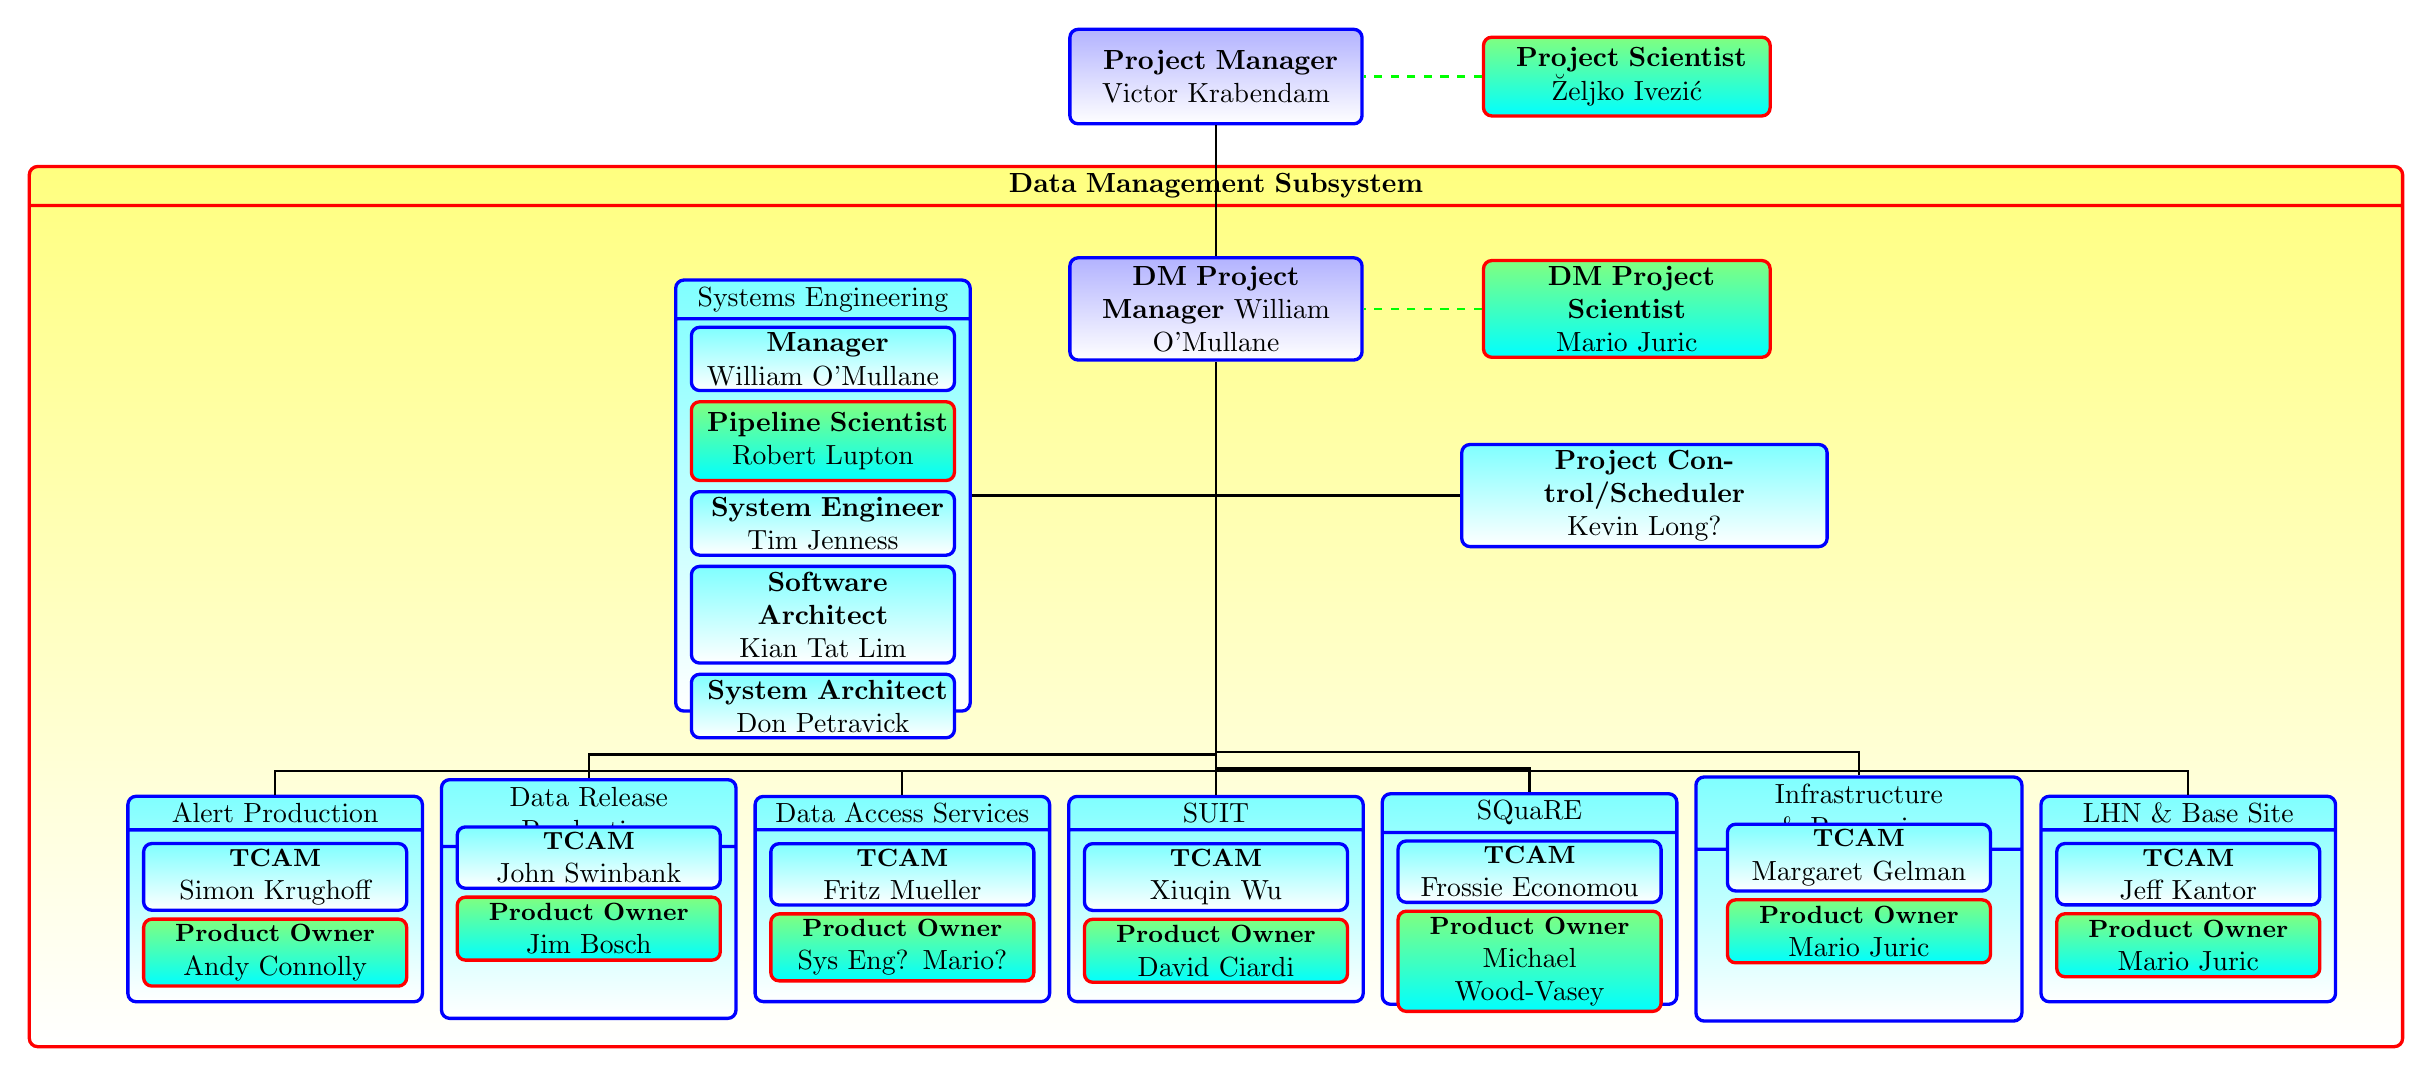
\begin{tikzpicture}[node distance=0mm]


    \node (dm) [arcbox, text width=30cm,  minimum height=10mm, rectangle split, rectangle split parts=2] 
	{ \textbf{Data Management Subsystem}
	   \nodepart{second} \vspace{105mm} 
	};

    \node (dmpm) [divbox, above=-2.5cm of dm.north] {\textbf{DM Project Manager} William O'Mullane};
    \node (pm) [divbox, above=.5cm of dm] {\textbf{ Project Manager} Victor Krabendam};
    \node (dmps) [psbox, right=1.5cm of dmpm] {\textbf{ DM Project Scientist}\\ Mario Juric};
    \node (ps) [psbox, right=1.5cm of pm] {\textbf{  Project Scientist}\\ \u{Z}eljko Ivezi\'c};

    \node (udmpm) [below=17mm of dmpm, text width=0mm]{};
% SYSTEM ENG
            \node (syseng) [mbox, text width=36mm, rectangle split, rectangle split parts=2, left=3.1cm of udmpm.north]
                {
                Systems Engineering
                \nodepart{second} \vspace{48mm}
                };
    \node (man) [mbox, below=6mm of syseng.north, text width=32mm] {\textbf{ Manager }\\ William O'Mullane };
    \node (pipe) [psbox, below=1mm of man, text width=32mm] {\textbf{ Pipeline Scientist}\\ Robert Lupton };
    \node (sysengineer) [mbox, below=1mm of pipe, text width=32mm] {\textbf{ System Engineer}\\ Tim Jenness };
    \node (softarc) [mbox, below=1mm of sysengineer, text width=32mm] {\textbf{ Software Architect}\\ Kian Tat Lim };
    \node (sysarc) [mbox, below=1mm of softarc, text width=32mm] {\textbf{ System Architect}\\ Don Petravick  };
%%%% end SYSENG

    \node (pcon) [mbox, right=3.1cm of udmpm.north , text width=45mm] {\textbf{Project Control/Scheduler }\\ Kevin Long?};
    %\node (al) [below=69mm of dmpm, text width=0mm]{};
    \dmnode[below=55mm of dmpm]{suit}{SUIT} {Xiuqin Wu  }{ David Ciardi } ;
    \dmnode[left=2mm of suit]{das}{Data Access Services}{Fritz Mueller}{Sys Eng? Mario?}  ;
    \dmnode[left=2mm of das]{drp}{Data Release Production}{John Swinbank}{Jim Bosch}  ;
    \dmnode[left=2mm of drp]{alerts}{Alert Production}{Simon Krughoff}{Andy Connolly}  ;
  \dmnode[right=2mm of suit]{square}{SQuaRE} {Frossie Economou}{ Michael Wood-Vasey} ;
    \dmnode[right=2mm of square,text width=40mm]{infra}{Infrastructure \& Processing} { Margaret Gelman   }{ Mario Juric} ;
    \dmnode[right=2mm of infra]{lhn}{LHN \& Base Site} { Jeff Kantor }{ Mario Juric } ;




   \draw[line] (dmpm.north) -- ++(0,0.8) -| (pm.south);

%dm lines second number is the proportional turning point of the line
   \draw[line] (alerts.north) -- ++(0,0.3) -| (dmpm.south);
   \draw[line] (drp.north) -- ++(0,0.3) -| (dmpm.south);
   \draw[line] (das.north) -- ++(0,0.3) -| (dmpm.south);
   \draw[line] (suit.north) -- ++(0,0.3) -| (dmpm.south);
   \draw[line] (square.north) -- ++(0,0.3) -| (dmpm.south);
   \draw[line] (infra.north) -- ++(0,0.3) -| (dmpm.south);
   \draw[line] (lhn.north) -- ++(0,0.3) -| (dmpm.south);

   \draw[line] (syseng.east) to (udmpm.north);
   \draw[line] (pcon.west) to (udmpm.north);
%science
   \draw[sline] (ps.west) to (pm.east);
   \draw[sline] (dmps.west) to (dmpm.east);

   

\end{tikzpicture}
\end{document}
